\documentclass{exam}
\pagestyle{headandfoot}
\firstpageheadrule
\runningheadrule
\firstpageheader{CT - Topic 3}{}{Sam Robbins}
\runningheader{CT - Topic 3}{How does Hardware Execture Software?}{Sam Robbins}
\firstpagefooter{}{}{}
\runningfooter{}{}{}
\renewcommand{\solutiontitle}{\noindent\textbf{Solution:}\par\noindent}


\printanswers
\usepackage{graphicx}
\marksnotpoints
\bracketedpoints
\pointsdroppedatright
\pointsinrightmargin
\begin{document}
\begin{center}
	\underline{\huge How Does Hardware Execute Software?}
\end{center}
\begin{questions}

\question[3]What is the Instruction Set Architecture (ISA) and what is the primary component of the ISA?
\begin{solution}[2in]
	The ISA is the interface between the hardware and software. The primary component of the ISA is its assembly language
\end{solution}

\question[6]Give three instructions of the MIPS (Microprocessor without Interlocked Pipeline Stages) ISA and explain carefully what they do.
\begin{solution}[2in]
	\begin{itemize}
		\item \texttt{lw \$s1, (\$s2)} - Register \$s1 takes the value of the memory location held in register \$s2
		\item \texttt{addi \$s1, \$s2, x} - register \$s1 takes the value of register \$s2 plus the number x
		\item \texttt{beq \$s1, \$s2, ,} - if the value of register \$s1 is equal to the value of the register \$s2 then go to memory location m
	\end{itemize}
\end{solution}

\question[2]What do we mean when we say that a MIPS (Microprocessor without Interlocked Pipeline Stages) instruction is 32 bits wide?
\begin{solution}[2in]
	There are 32 bits in the MIPS instruction
\end{solution}

\question[6]What is a process control block (PCB) and what is one used for by the operating system? Name 3 items in a PCB.
\begin{solution}[2in]
	\begin{itemize}
		\item \textbf{Process control block(PCB)} - a data structure that the kernel uses in order to manage a process
		\item It is used so that the current situation of any process is fully understood, this means that the CPU can better handle processes
		\item Components
		\begin{itemize}
			\item the process's unique ID
			\item The current state of the process
			\item CPU scheduling information such as the process priority
		\end{itemize}
	\end{itemize}
\end{solution}


\newpage
\question[6]What are the three types that MIPS instructions are partitioned into? Briefly describe these types.
\begin{solution}[2in]
	\begin{itemize}
		\item I type instructions
		\begin{itemize}
			\item Involve data transfer
			\item 6 bit op code
			\item 5 bit Rs (Source Register)
			\item 5 bit Rd (Destination Register)
			\item 16 bit address
		\end{itemize}
		\item R type instructions
		\begin{itemize}
			\item Work on registers
			\item 6 bit op code
			\item 5 bit Rs1 (first source register)
			\item 5 bit Rs2 (Second source register)
			\item 5 bit Rd (Destination Register)
			\item 5 bit shift (The shift amount for shift instructions)
			\item 6 bit funct (A supplement for opcode for some instructions)
		\end{itemize}
		\item J type instructions
		\begin{itemize}
			\item Involve jumps
			\begin{itemize}
				\item 6 bit opcode
				\item 26 bit address
			\end{itemize}
		\end{itemize}
	\end{itemize}
\end{solution}

\question[4]Detail four different functions of the operating system.
\begin{solution}[2in]
	\begin{itemize}
		\item Virtualises a machine
		\begin{itemize}
			\item Provides abstractions that present clean interfaces to make the computer easier to use.
		\end{itemize}
		\item Starts and stops programs
		\begin{itemize}
			\item Ensures that when a program is stopped, it's memory is freed up
		\end{itemize}
		\item Manages memory
		\begin{itemize}
			\item Ensures programs can still run, even if the memory they request is in use.
		\end{itemize}
		\item Handles input/output
		\begin{itemize}
			\item Handles interrupts from inputs and outputs so that they don't have to wait for the processor to finish what it is doing.
		\end{itemize}
	\end{itemize}
\end{solution}
\newpage
\question[1]What is data security (in the context of operating systems)?
\begin{solution}[2in]
Ensuring that the memory allocated to each program is kept separate and secure from other programs
\end{solution}

\question[2]What is virtualization (in the context of operating systems)?
\begin{solution}[2in]
Providing abstractions that present clean interfaces to make the computer easier to use
\end{solution}

\question[4]Explain what an interrupt is and how the operating system uses interrupts to deal with peripheral devices that operate much more slowly than the CPU.
\begin{solution}[2in]
	\begin{itemize}
		\item An interrupt is an input from the user which should be handled immediately by the cpu
		\item The operating system ensures the actions are coordinated
		\item Ensures no programs end up being closed because a mouse is clicked
	\end{itemize}
\end{solution}

\question[5]What is process within an operating system and what are the two essential elements of a process? Is it the case that an operating system for a CPU with one processor can only have one process?
\begin{solution}[2in]
\begin{itemize}
	\item Process - Each executing program
	\item A process consists of
	\begin{itemize}
		\item \textbf{Thread} - A sequence of instructions in the context of a sequential execution
		\item \textbf{Address space} - Consists of some memory locations that the corresponding process can read from and write to
	\end{itemize}
	\item Multiple processes can be run on one processor, providing there is no mutual exclusion 
\end{itemize}
\end{solution}

\question[6]Explain the principle of mutual exclusion and give an illustration to show that ensuring mutual exclusion is important.
\begin{solution}[2in]
\begin{itemize}
	\item \textbf{Mutual Exclusion} - Ensuring that two threads are not in the critical selection at the same time
	\item \textbf{Critical Selection} - Exclusive access to some shared resource such as memory location
	\item  Two threads have access to the same counter, and each want to increment the counter, depending on how the read, increment, store is handled, the result will be different
\end{itemize}
\end{solution}

\question[3]Explain how the principle of virtual memory works. Why is virtual memory required?
\begin{solution}[2in]
\begin{itemize}
	\item Moving memory backwards and forwards between RAM and the hard disk as and when required
	\item Virtual memory is required when there is insufficient RAM to store what all the running programs wish to store in RAM
	\item Lower priority processes are moved to hard disk first
\end{itemize}
\end{solution}

\question[10]Describe the life-cycle of processes within the operating system (be sure to explain each component of the life-cycle).
\begin{solution}[2in]
\begin{itemize}
	\item \textbf{new}: the process being created
	\item \textbf{ready:} the process not executing on the CPU but is ready to execute
	\item \textbf{running:} the process is executing on the CPU
	\item \textbf{blocked:} the process is waiting for an event (and so not executable)
	\item \textbf{exit:} the process has finished
\end{itemize}
There are the following state transitions
\begin{itemize}
	\item \textbf{admit:} the control overheads as regards a process have been set up and the process is moved to the run queue
	\item \textbf{dispatch:} the scheduler allocates the CPU to an executable process
	\item \textbf{timeout/yield:} the executing process is forced to/volunteers to release access to cpu
	\item \textbf{event-wait:} a process is waiting for an input/output event, for example, and gives up access to the cpu
	\item \textbf{event:} an event occurs and wakes up a process
	\item \textbf{release:} a process terminates and releases access to the CPU and other resources
\end{itemize}
\end{solution}


\newpage
\question[5]Explain the principle of context switching with regard to process control blocks.
\begin{solution}[2in]
\textbf{Context switching} - Where the operating system pauses one process and resumes another process
\begin{center}
	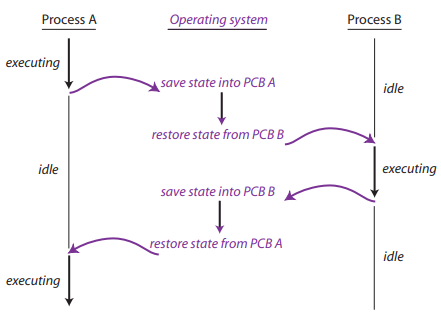
\includegraphics[scale=0.7]{context_switching}
\end{center}
\end{solution}

\question[2]Give two illustrations of principles of Computational Thinking in the context of instruction set architectures and operating systems.
\begin{solution}[2in]
	\begin{itemize}
		\item Tessellation - Changing the model of processes to "cells", each with their own guarantees of resources
		\item Technological advances such as multi-core, cloud computing and embedded systems
	\end{itemize}
\end{solution}


\end{questions}



\end{document}